\section{Программирование}

\subsection{Заполнение базы данных}

Создание таблиц базы данных выполняется SQL-скриптом, приведённым в приложении~\ref{app:init-sql}. Заполнение базы данных выполняется программой на Node.js и TypeScript, исходный код которой приведён в приложении~\ref{app:seed-ts}. При заполнении сначала создаются справочные таблицы, затем таблицы предметной области, зависящие от них по внешним ключам.

В результате выполнения программы заполнения были получены количества записей, приведённые в таблице~\ref{table:programming-counts}.

\begin{table}[H]
    \centering
    \caption{Количество записей в таблицах базы данных}
    \label{table:programming-counts}
    \begin{tblr}{
        colspec = {|X[l]|X[r]|},
        row{1} = {font=\bfseries},
        row{13} = {font=\bfseries},
        hlines,
        vlines,
    }
        Название таблицы & Количество записей \\
        \mintinline{text}{Category} & 12 \\
        \mintinline{text}{Weight} & 9 \\
        \mintinline{text}{Slope} & 3 \\
        \mintinline{text}{Extension} & 5 \\
        \mintinline{text}{Writing_direction} & 2 \\
        \mintinline{text}{Script_type} & 3 \\
        \mintinline{text}{Format} & 5 \\
        \mintinline{text}{Language} & 40 \\
        \mintinline{text}{Font_family} & 210 \\
        \mintinline{text}{Typeface} & 4217 \\
        \mintinline{text}{Symbol} & 581014 \\
        Всего записей в БД & 585498 \\
    \end{tblr}
\end{table}

\subsection{Запросы}

Для проверки работы базы данных были составлены SQL-запросы, соответствующие основным пользовательским операциям. Лист проверки выполнения запросов представлен на рисунке~\ref{fig:query-check-list}. Тексты запросов хранятся в отдельных SQL-файлах в каталоге \mintinline{text}{src/queries}. Для построения визуализаций планов выполнения используется сервис Dalibo Explain\footnote{\url{https://explain.dalibo.com/}}: в него можно загрузить результат выполнения команды \mintinline{sql}{EXPLAIN (ANALYZE, BUFFERS, FORMAT JSON)} для нужного запроса.

\screenshot[fig:query-check-list][0.9]{img/quaries.pdf}{Лист проверки выполнения запросов}

Время планирования и выполнения запросов было получено с помощью команды \mintinline{sql}{EXPLAIN (ANALYZE, BUFFERS)}. Результаты измерений приведены в таблице~\ref{table:query-times}.

\begin{table}[H]
    \centering
    \caption{Время планирования и выполнения запросов}
    \label{table:query-times}
    \begin{tblr}{
        colspec = {|X[c]|X[r]|X[r]|},
        row{1} = {font=\bfseries},
        hlines,
        vlines,
    }
        Номер запроса & Время планирования, мс & Время выполнения, мс \\
        1 & 0.628 & 0.943 \\
        2 & 0.626 & 766.385 \\
        3 & 0.260 & 348.445 \\
        4 & 0.234 & 105.751 \\
        5 & 3.739 & 1.374 \\
        6 & 0.396 & 7.491 \\
        7 & 0.239 & 1.308 \\
        8 & 0.349 & 109.254 \\
        9 & 1.763 & 1.729 \\
    \end{tblr}
\end{table}

В формулах далее используются обозначения: $C$ --- \mintinline{text}{Category}, $FF$ --- \mintinline{text}{Font_family}, $T$ --- \mintinline{text}{Typeface}, $F$ --- \mintinline{text}{Format}, $L$ --- \mintinline{text}{Language}, $S$ --- \mintinline{text}{Symbol}, $W$ --- \mintinline{text}{Weight}. Символ $\bowtie$ обозначает соединение таблиц по соответствующим внешним ключам, $\underset{L}{\bowtie}$ --- левое внешнее соединение, $\sigma$ --- выборку, $\pi$ --- проекцию, $\gamma$ --- группировку с агрегированием.

\subsubsection{Запрос 1}

Найти начертания, относящиеся к категории $A$, у которых присутствует символ $B$, поддерживаемый начертанием $C$ для того же языка.

\[
\begin{aligned}
Q_C &= \pi_{S_C.value,S_C.id\_Language}
\left(\sigma_{T_C.name=C \land S_C.value=B}(T_C \bowtie S_C)\right),\\
R_1 &= \pi_{T.id,T.name}
\left(
    \sigma_{\substack{C.name=A \land S.value=Q_C.value\\ S.id\_Language=Q_C.id\_Language}}
    (T \bowtie FF \bowtie C \bowtie S \bowtie Q_C)
\right).
\end{aligned}
\]

Текст запроса~1 приведён в листинге~\ref{lst:query-01}, результат выполнения показан на рисунке~\ref{fig:query-01-result}, схема плана выполнения --- на рисунке~\ref{fig:query-01-plan}.

\captionof{listing}{Запрос 1}
\label{lst:query-01}
\vspace{-10pt}
\inputminted[linenos, numbersep=10pt, firstnumber=1, fontsize=\small]{sql}{../src/queries/query_01.sql}

Запрос сначала находит заданный символ у исходного начертания $C$, затем ищет такие же символы в начертаниях категории $A$ для того же языка. В результате возвращаются подходящие начертания.

\screenshot[fig:query-01-plan][0.95]{img/query-01-plan.png}{План выполнения запроса 1}

План выполнения запроса 1 строится от выборки исходного начертания и его символа. Затем по индексам находятся связанные гарнитура, категория и символы других начертаний. После соединения таблиц PostgreSQL оставляет только уникальные подходящие начертания.

\screenshot[fig:query-01-result][0.65]{img/query-01-result.png}{Результат выполнения запроса 1}

\subsubsection{Запрос 2}

Посчитать число языков, в которых присутствует формат $A$ и которые относятся к категории $C$.

\[
R_2 =
\gamma_{\operatorname{count\_distinct}(L.id)}
\left(
    \sigma_{F.name=A \land C.name=C}
    (L \bowtie S \bowtie T \bowtie F \bowtie FF \bowtie C)
\right)
\]

Текст запроса~2 приведён в листинге~\ref{lst:query-02}, результат выполнения показан на рисунке~\ref{fig:query-02-result}, схема плана выполнения --- на рисунке~\ref{fig:query-02-plan}.

\captionof{listing}{Запрос 2}
\label{lst:query-02}
\vspace{-10pt}
\inputminted[linenos, numbersep=10pt, firstnumber=1, fontsize=\small]{sql}{../src/queries/query_02.sql}

Запрос выбирает языки, связанные с начертаниями заданного формата и гарнитурами заданной категории. Затем он считает количество различных языков, чтобы один язык не учитывался несколько раз.

\screenshot[fig:query-02-plan][0.95]{img/query-02-plan.png}{План выполнения запроса 2}

План выполнения запроса 2 последовательно соединяет таблицы языков, символов, начертаний, форматов, гарнитур и категорий. После фильтрации по формату и категории выполняется агрегирование с подсчётом различных языков.

\screenshot[fig:query-02-result][0.55]{img/query-02-result.png}{Результат выполнения запроса 2}

\subsubsection{Запрос 3}

Для каждого формата посчитать число начертаний и число символов алфавита. Полученные значения используются для построения гистограммы.

\[
R_3 =
\gamma_{F.id,F.name;\ \operatorname{count\_distinct}(T.id),\operatorname{count}(S.id)}
(F \underset{L}{\bowtie} T \underset{L}{\bowtie} S)
\]

Текст запроса~3 приведён в листинге~\ref{lst:query-03}, результат выполнения показан на рисунке~\ref{fig:query-03-result}, гистограмма по полученным данным --- на рисунке~\ref{fig:query-03-histogram}, схема плана выполнения --- на рисунке~\ref{fig:query-03-plan}.

\captionof{listing}{Запрос 3}
\label{lst:query-03}
\vspace{-10pt}
\inputminted[linenos, numbersep=10pt, firstnumber=1, fontsize=\small]{sql}{../src/queries/query_03.sql}

Запрос группирует данные по форматам. Для каждого формата считается число различных начертаний и общее число связанных символов.

\screenshot[fig:query-03-plan][0.75]{img/query-03-plan.png}{План выполнения запроса 3}

План выполнения запроса 3 соединяет форматы с начертаниями и символами, сохраняя форматы даже при отсутствии связанных строк. После этого PostgreSQL группирует строки по формату и считает агрегаты.

\screenshot[fig:query-03-result][0.75]{img/query-03-result.png}{Результат выполнения запроса 3}

\begin{figure}[H]
    \centering
    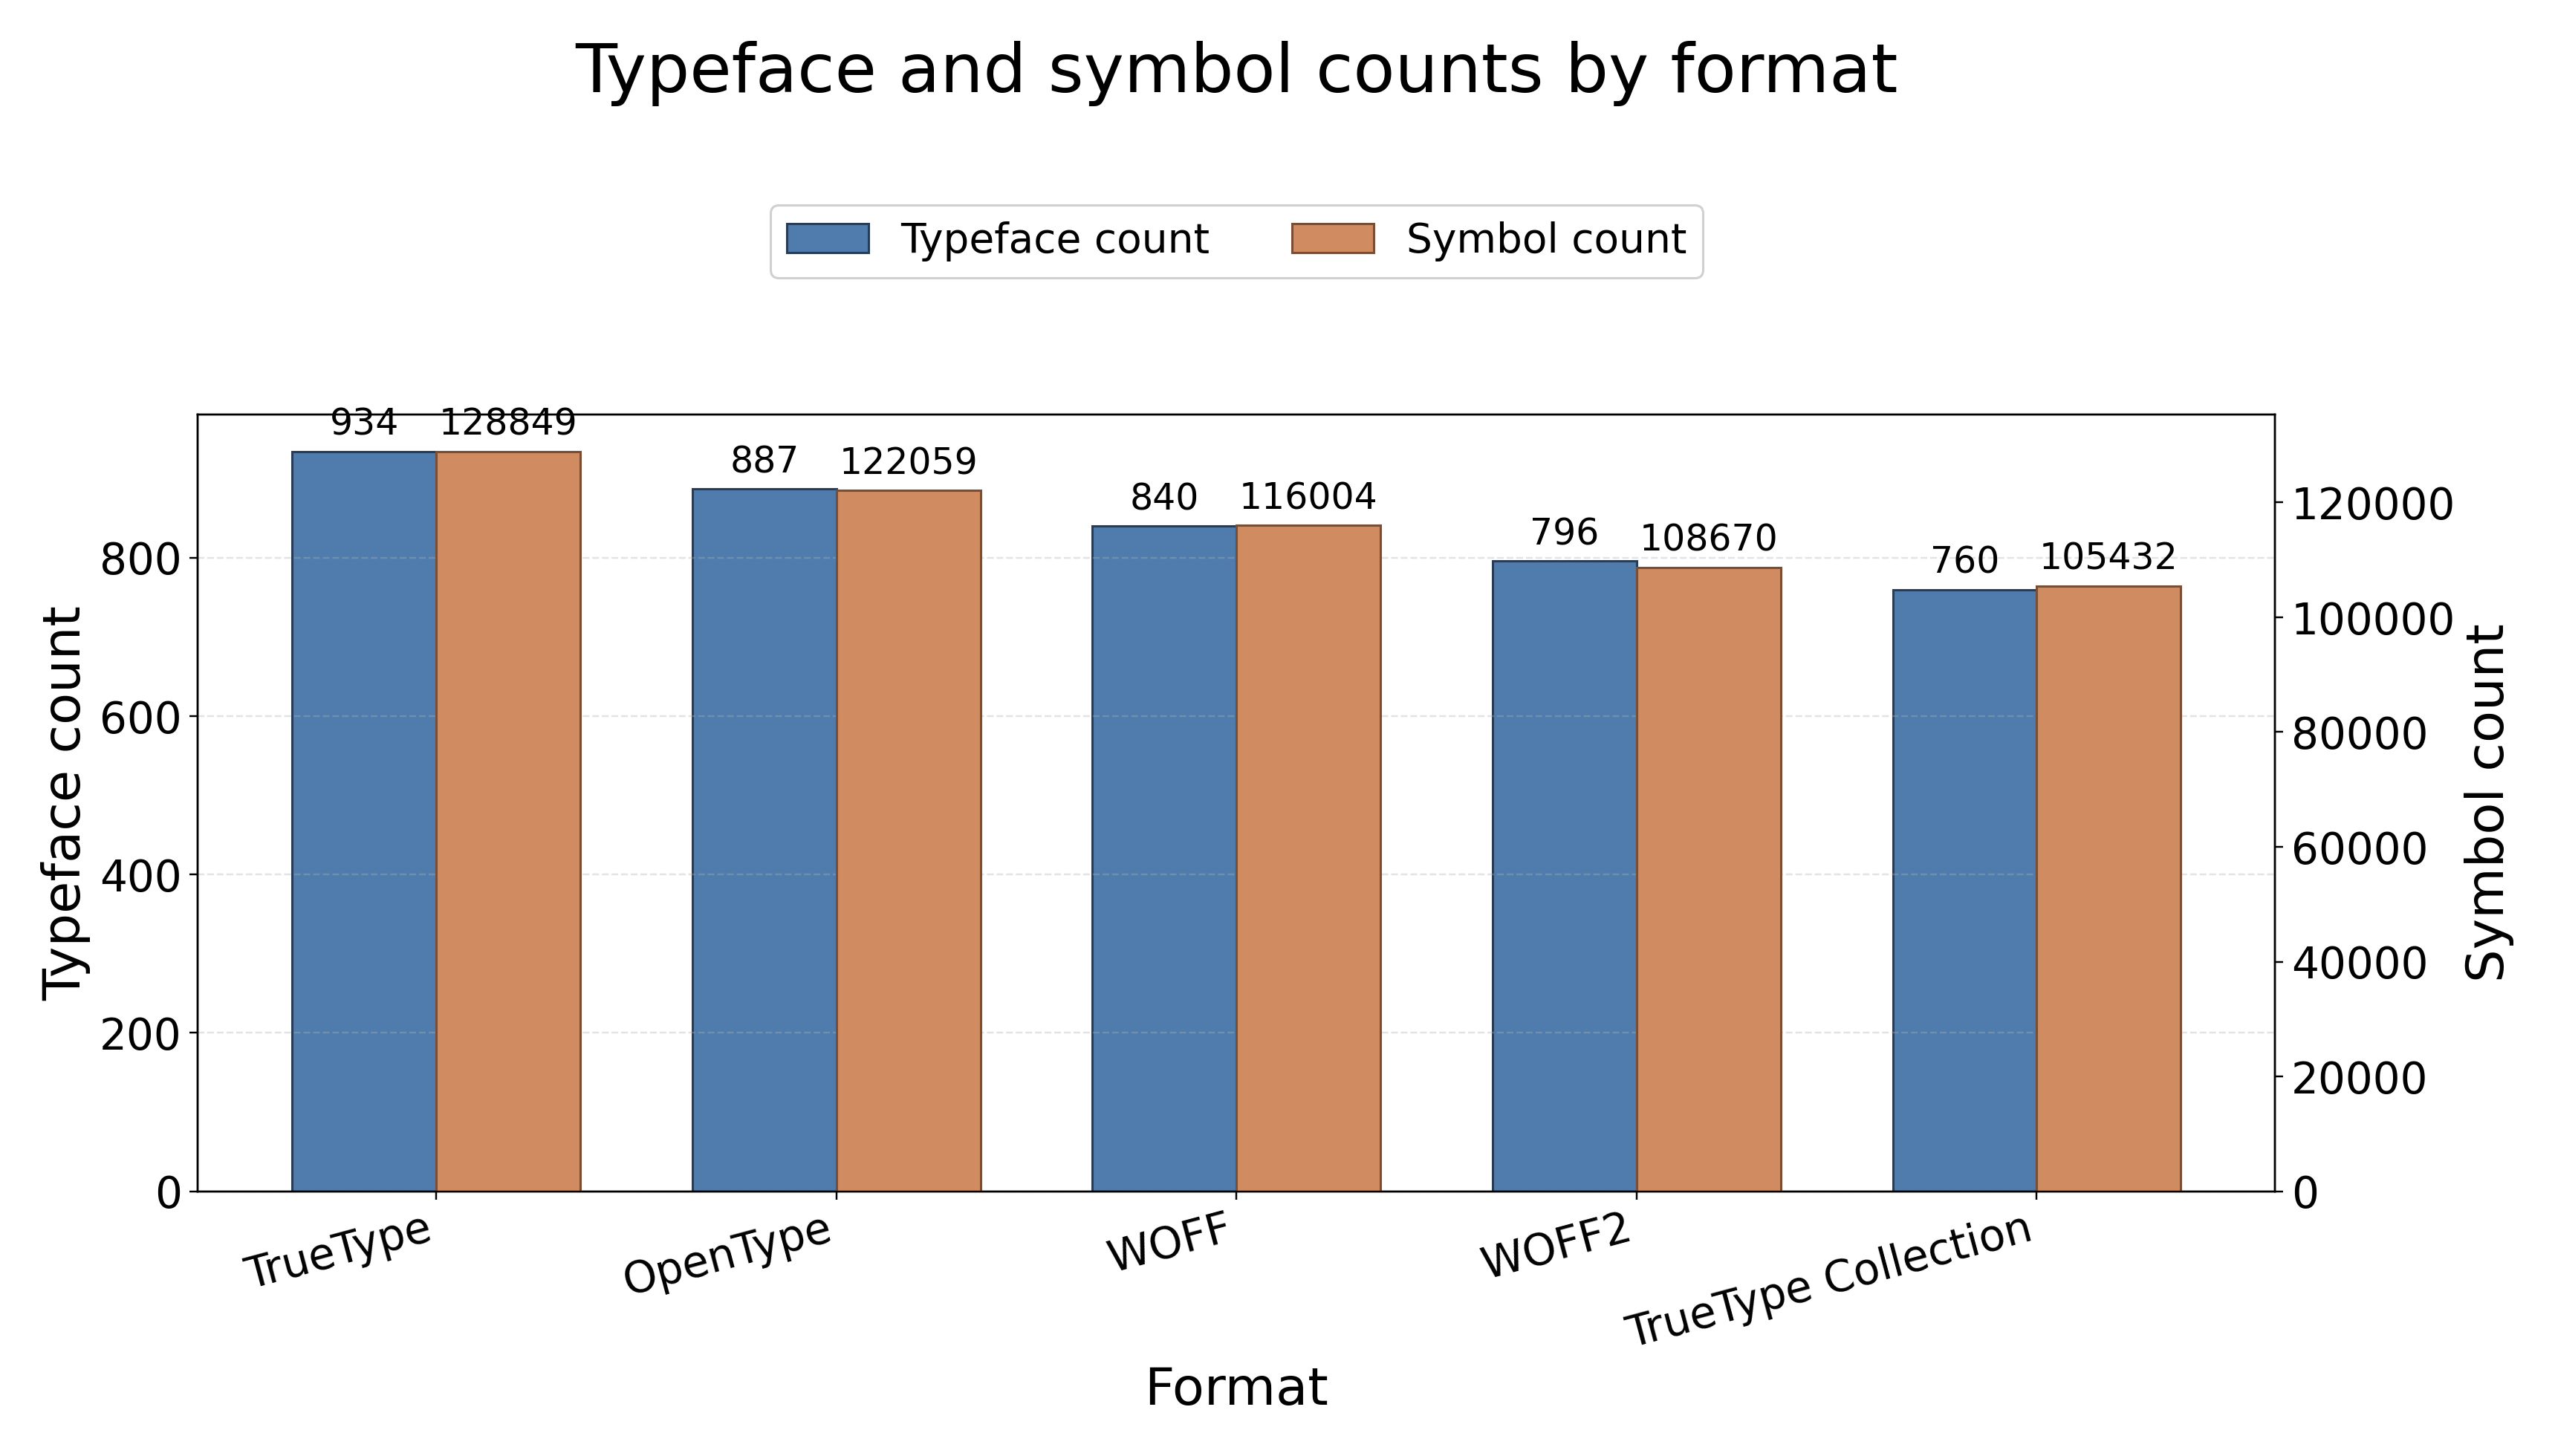
\includegraphics[width=0.95\textwidth]{histograms/query-03-histogram.png}
    \caption{Гистограмма по результатам запроса 3}
    \label{fig:query-03-histogram}
\end{figure}

Гистограмма показывает, что больше всего записей связано с форматом \mintinline{text}{TrueType}.

\subsubsection{Запрос 4}

Посчитать число начертаний с одинаковым числом символов. Полученные значения используются для построения гистограммы.

\[
\begin{aligned}
Q &= \gamma_{T.id;\ \operatorname{count}(S.id) \rightarrow symbol\_count}
(T \underset{L}{\bowtie} S),\\
R_4 &= \gamma_{symbol\_count;\ \operatorname{count}(T.id) \rightarrow typeface\_count}(Q).
\end{aligned}
\]

Текст запроса~4 приведён в листинге~\ref{lst:query-04}, гистограмма по полученным данным показана на рисунке~\ref{fig:query-04-histogram}, схема плана выполнения --- на рисунке~\ref{fig:query-04-plan}.

\captionof{listing}{Запрос 4}
\label{lst:query-04}
\vspace{-10pt}
\inputminted[linenos, numbersep=10pt, firstnumber=1, fontsize=\small]{sql}{../src/queries/query_04.sql}

Запрос сначала считает количество символов для каждого начертания. Затем полученные значения группируются повторно, чтобы определить, сколько начертаний имеют одинаковое число символов.

\screenshot[fig:query-04-plan][0.75]{img/query-04-plan.png}{План выполнения запроса 4}

План выполнения запроса 4 начинается с соединения начертаний и символов. Затем выполняется первая группировка по начертанию, а после неё вторая группировка по найденному числу символов.

\begin{figure}[H]
    \centering
    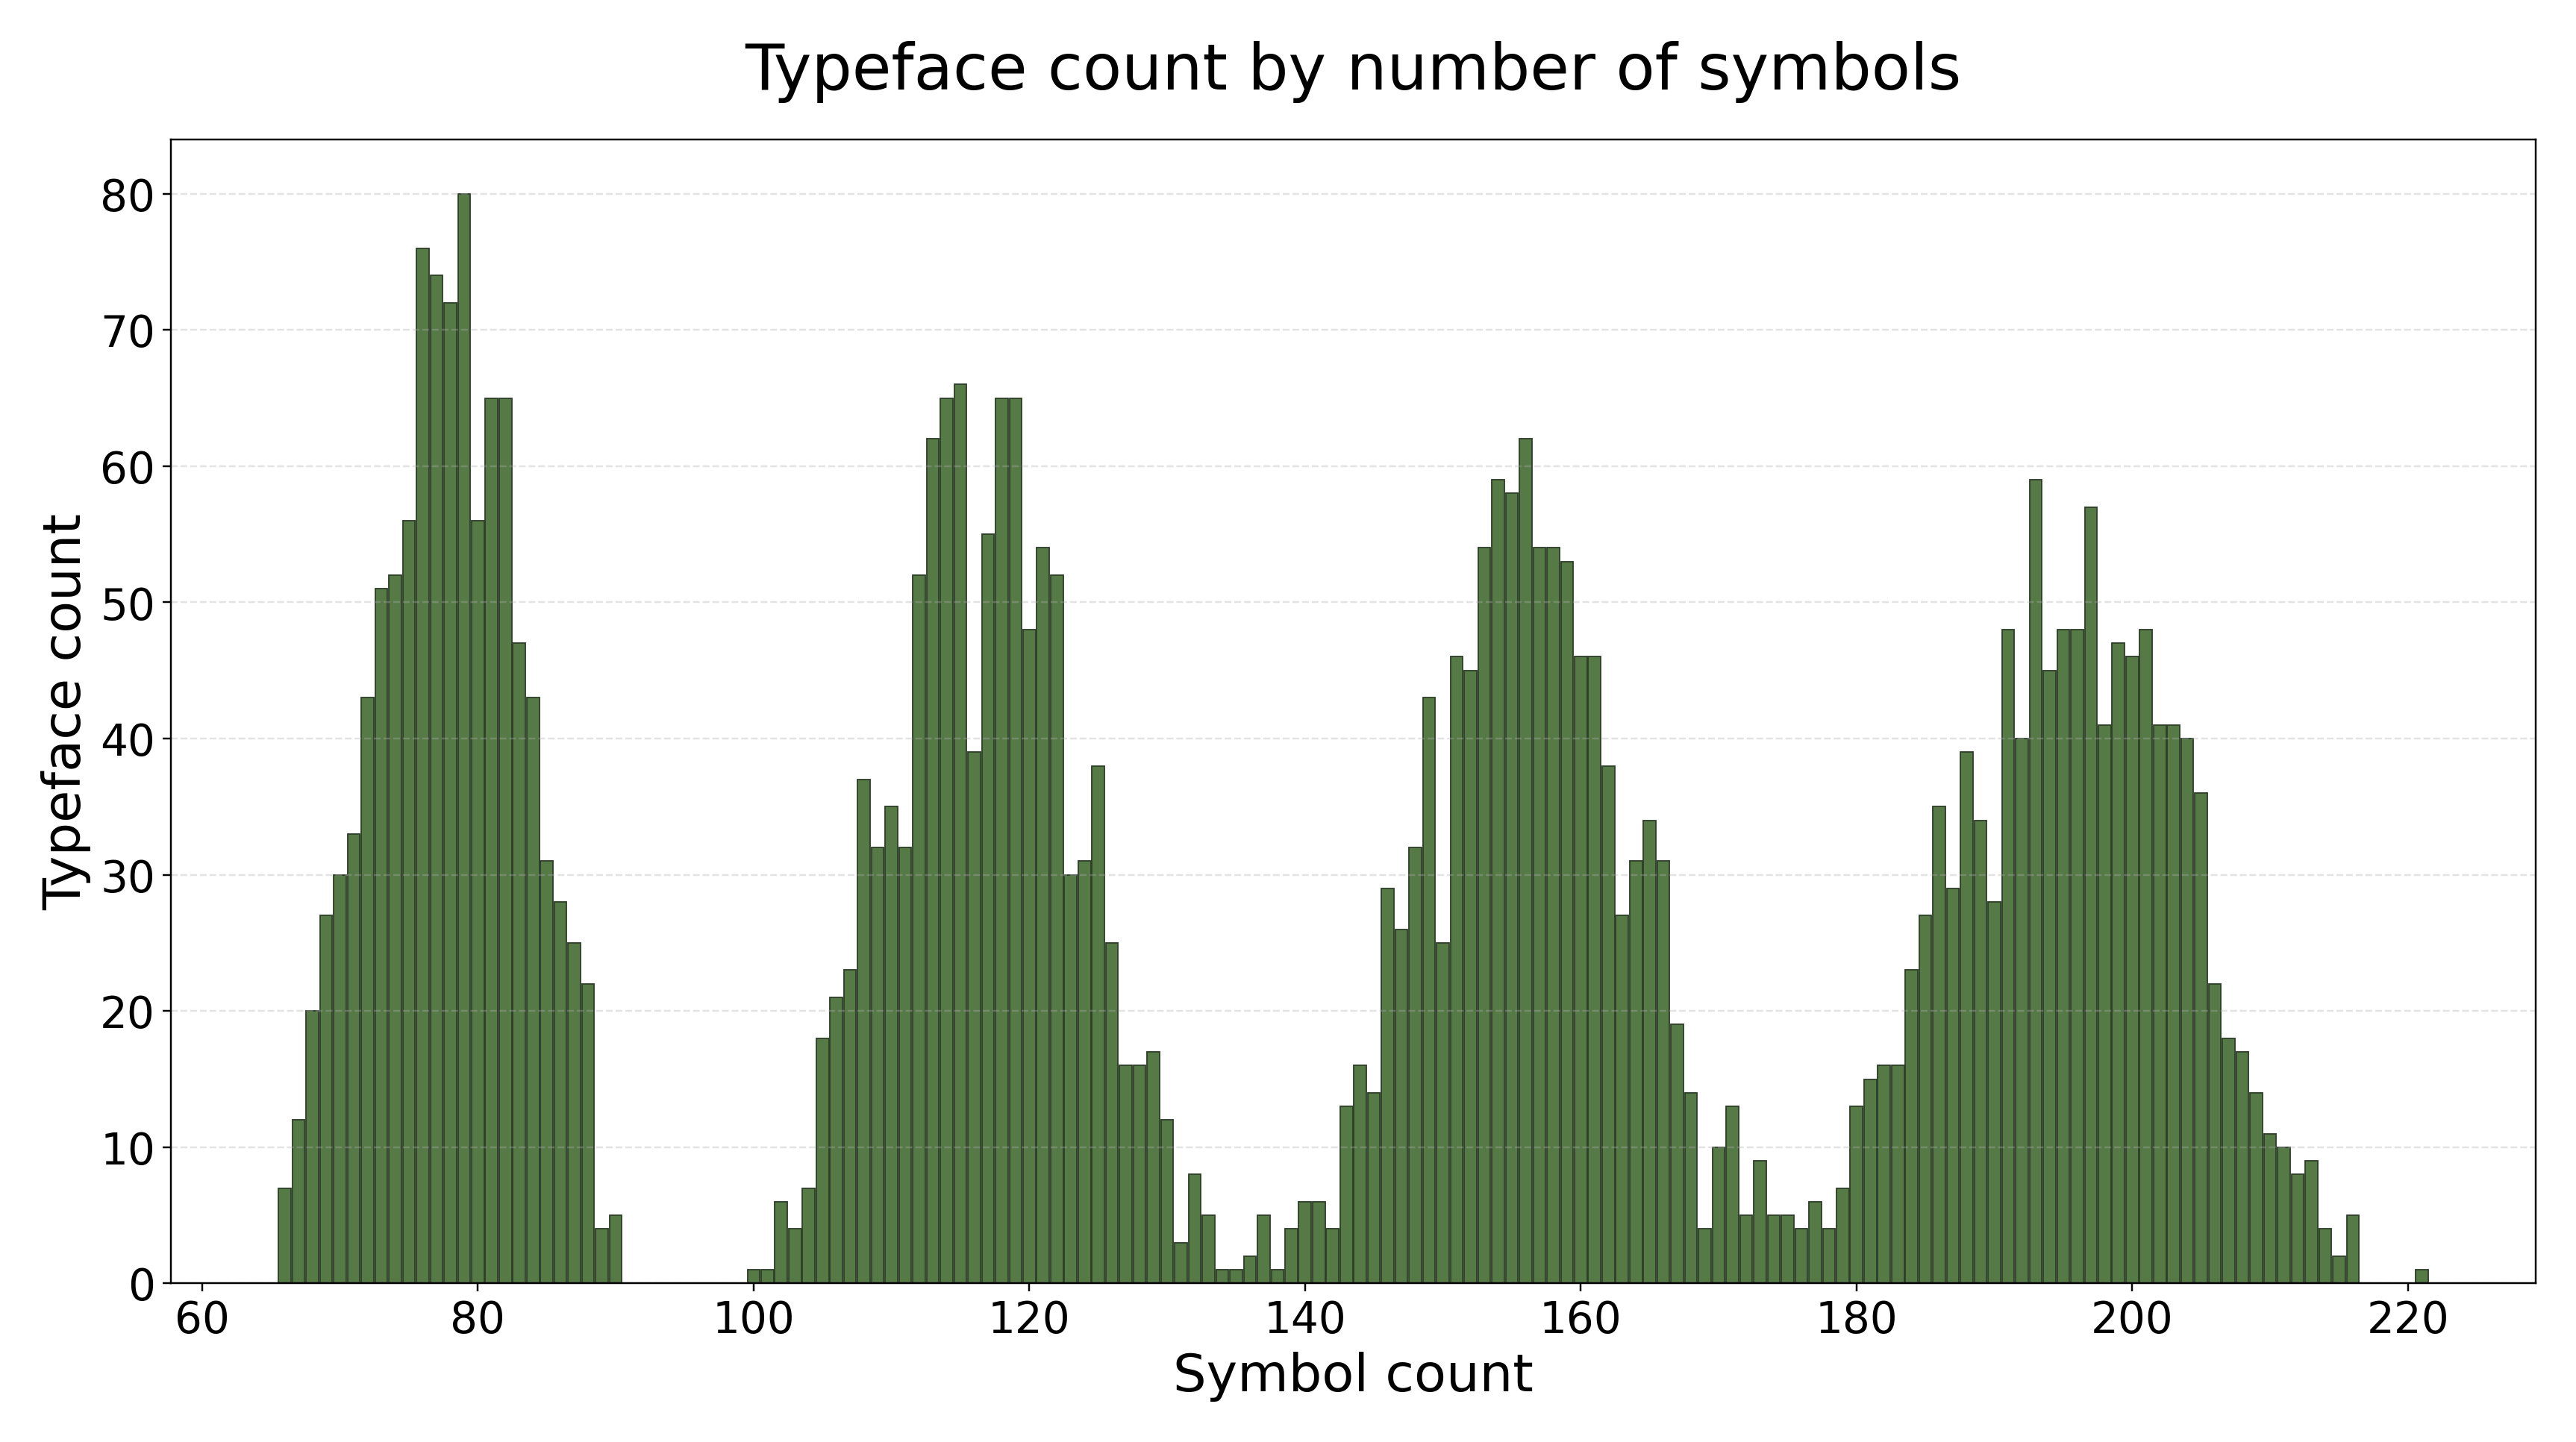
\includegraphics[width=0.95\textwidth]{histograms/query-04-histogram.png}
    \caption{Гистограмма по результатам запроса 4}
    \label{fig:query-04-histogram}
\end{figure}

Итоговые данные показаны на гистограмме.

\subsubsection{Запрос 5}

Найти категории с наибольшим числом гарнитур и наименьшим числом гарнитур.

\[
\begin{aligned}
Q &= \gamma_{C.name;\ \operatorname{count\_distinct}(FF.id) \rightarrow category\_count}
(C \bowtie FF),\\
R_5 &= \sigma_{\substack{category\_count=\max(Q.category\_count)\\
\lor\ category\_count=\min(Q.category\_count)}}(Q).
\end{aligned}
\]

Текст запроса~5 приведён в листинге~\ref{lst:query-05}, результат выполнения показан на рисунке~\ref{fig:query-05-result}, схема плана выполнения --- на рисунке~\ref{fig:query-05-plan}.

\captionof{listing}{Запрос 5}
\label{lst:query-05}
\vspace{-10pt}
\inputminted[linenos, numbersep=10pt, firstnumber=1, fontsize=\small]{sql}{../src/queries/query_05.sql}

Запрос считает число гарнитур в каждой категории. Затем из полученного набора выбираются категории с минимальным и максимальным значением.

\screenshot[fig:query-05-plan][0.75]{img/query-05-plan.png}{План выполнения запроса 5}

План выполнения запроса 5 соединяет категории с гарнитурами, группирует строки по категории и считает количество гарнитур. После этого оконные функции находят минимальное и максимальное значения, а внешний запрос оставляет только эти строки.

\screenshot[fig:query-05-result][0.75]{img/query-05-result.png}{Результат выполнения запроса 5}

\subsubsection{Запрос 6}

Найти языки, в которых отсутствует насыщенность $A$.

\[
R_6 =
\pi_{L.id,L.name}(L) -
\pi_{L.id,L.name}\left(\sigma_{W.name=A}(L \bowtie S \bowtie T \bowtie W)\right)
\]

Текст запроса~6 приведён в листинге~\ref{lst:query-06}, результат выполнения показан на рисунке~\ref{fig:query-06-result}, схема плана выполнения --- на рисунке~\ref{fig:query-06-plan}.

\captionof{listing}{Запрос 6}
\label{lst:query-06}
\vspace{-10pt}
\inputminted[linenos, numbersep=10pt, firstnumber=1, fontsize=\small]{sql}{../src/queries/query_06.sql}

Запрос перебирает языки и для каждого проверяет, есть ли в нём начертания с насыщенностью $A$. В результат попадают только языки, для которых такая связанная запись не найдена.

\screenshot[fig:query-06-plan][0.75]{img/query-06-plan.png}{План выполнения запроса 6}

План выполнения запроса 6 использует проверку отсутствия строк: для языков ищутся связанные символы, начертания и насыщенности. В тестовых данных словарь насыщенностей заполнен полностью, поэтому языков без заданной насыщенности не найдено.

\screenshot[fig:query-06-result][0.6]{img/query-06-result.png}{Результат выполнения запроса 6}

\subsubsection{Запрос 7}

Найти форматы, в которых больше начертаний, чем в формате $A$.

\[
\begin{aligned}
B &= \operatorname{count}\left(\sigma_{F.name=A}(T \bowtie F)\right),\\
Q &= \gamma_{F.id,F.name;\ \operatorname{count}(T.id) \rightarrow typeface\_count}
(F \underset{L}{\bowtie} T),\\
R_7 &= \sigma_{typeface\_count>B}(Q).
\end{aligned}
\]

Текст запроса~7 приведён в листинге~\ref{lst:query-07}, результат выполнения показан на рисунке~\ref{fig:query-07-result}, схема плана выполнения --- на рисунке~\ref{fig:query-07-plan}.

\captionof{listing}{Запрос 7}
\label{lst:query-07}
\vspace{-10pt}
\inputminted[linenos, numbersep=10pt, firstnumber=1, fontsize=\small]{sql}{../src/queries/query_07.sql}

Запрос сначала считает количество начертаний в базовом формате \mintinline{text}{WOFF2}. Затем он считает начертания для остальных форматов и оставляет только те, где значение больше.

\screenshot[fig:query-07-plan][0.95]{img/query-07-plan.png}{План выполнения запроса 7}

План выполнения запроса 7 выполняет два агрегирования: одно для базового формата, второе для всех форматов. После сравнения агрегатов в результате остаются \mintinline{text}{TrueType}, \mintinline{text}{OpenType} и \mintinline{text}{WOFF}.

\screenshot[fig:query-07-result][0.6]{img/query-07-result.png}{Результат выполнения запроса 7}

\subsubsection{Запрос 8}

Для каждой категории и каждого языка посчитать число символов. Для вывода используются первые 10 языков; результат предназначен для построения гистограммы.

\[
\begin{aligned}
Q &= (C \times L_{1..10}) \underset{L}{\bowtie} FF
\underset{L}{\bowtie} T \underset{L}{\bowtie} S,\\
R_8 &= \gamma_{C.id,C.name,L.id,L.name;\ \operatorname{count}(S.id)}(Q).
\end{aligned}
\]

Текст запроса~8 приведён в листинге~\ref{lst:query-08}, гистограммы по полученным данным показаны на рисунках~\ref{fig:query-08-histogram} и~\ref{fig:query-08-histogram-3d}, схема плана выполнения --- на рисунке~\ref{fig:query-08-plan}.

\captionof{listing}{Запрос 8}
\label{lst:query-08}
\vspace{-10pt}
\inputminted[linenos, numbersep=10pt, firstnumber=1, fontsize=\small]{sql}{../src/queries/query_08.sql}

Запрос строит пары из категорий и первых десяти языков. Для каждой пары считается число символов, связанных через гарнитуры и начертания.

\screenshot[fig:query-08-plan][0.75]{img/query-08-plan.png}{План выполнения запроса 8}

План выполнения запроса 8 сначала формирует пары «категория --- язык», затем присоединяет гарнитуры, начертания и символы. Внешние соединения нужны, чтобы сохранить пары даже без связанных символов.

\begin{figure}[H]
    \centering
    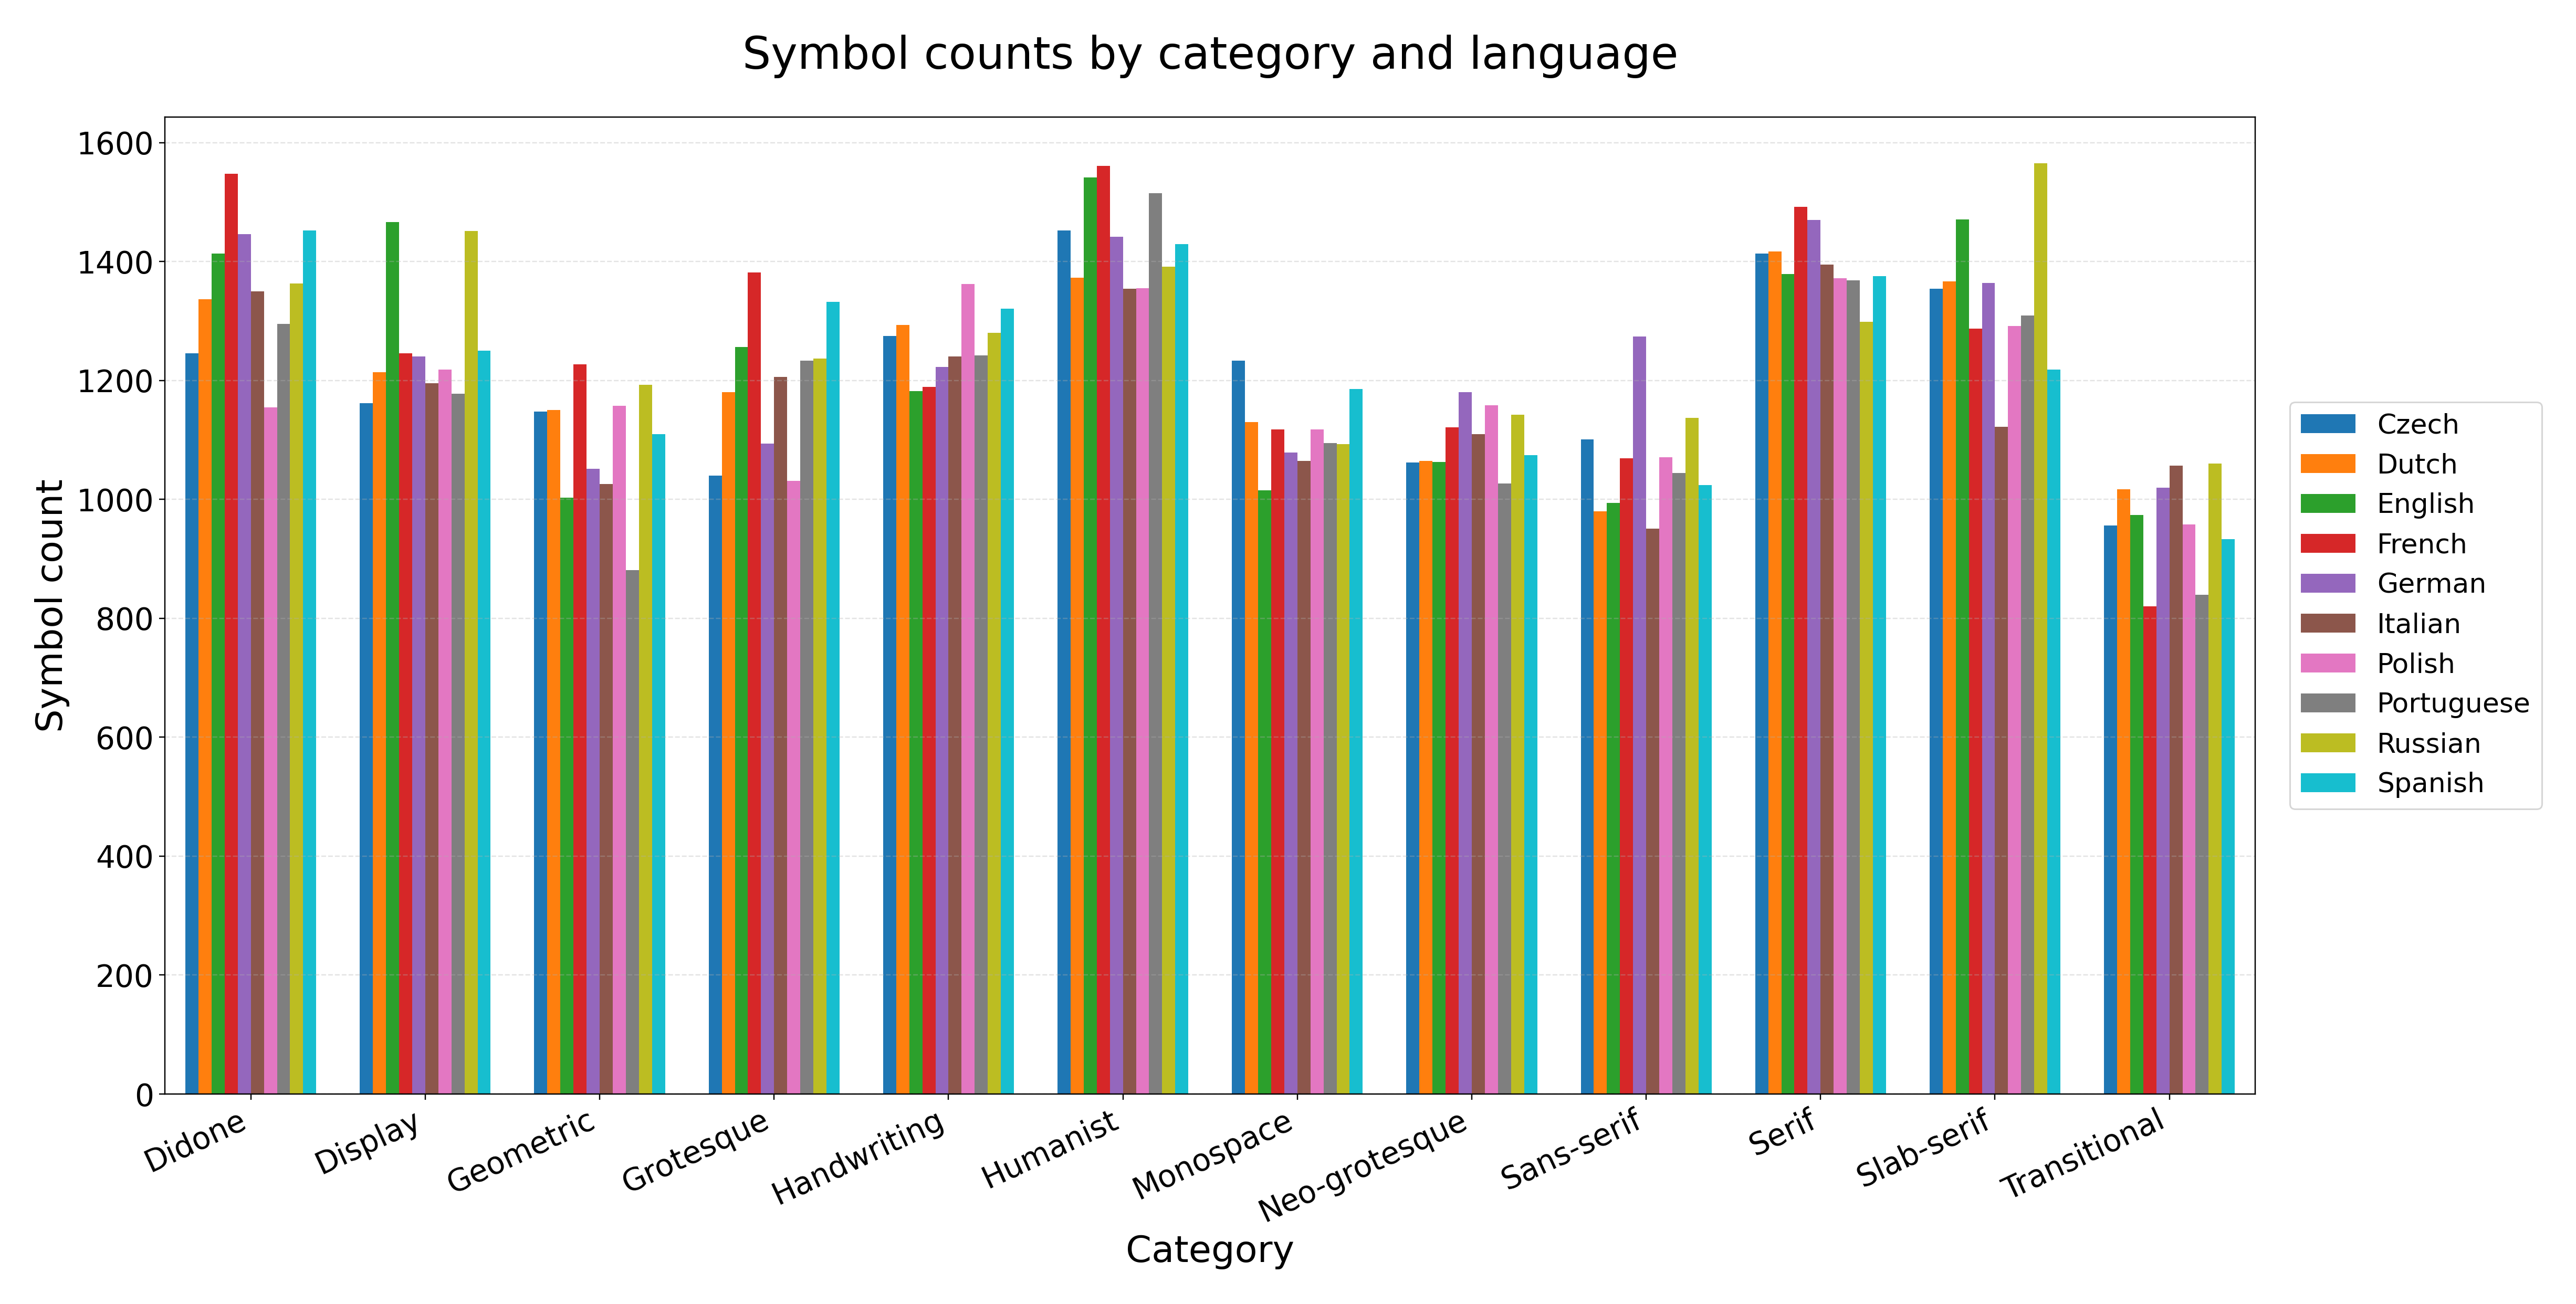
\includegraphics[width=\textwidth]{histograms/query-08-histogram.png}
    \caption{Двумерная гистограмма по результатам запроса 8}r
    \label{fig:query-08-histogram}
\end{figure}

\begin{figure}[H]
    \centering
    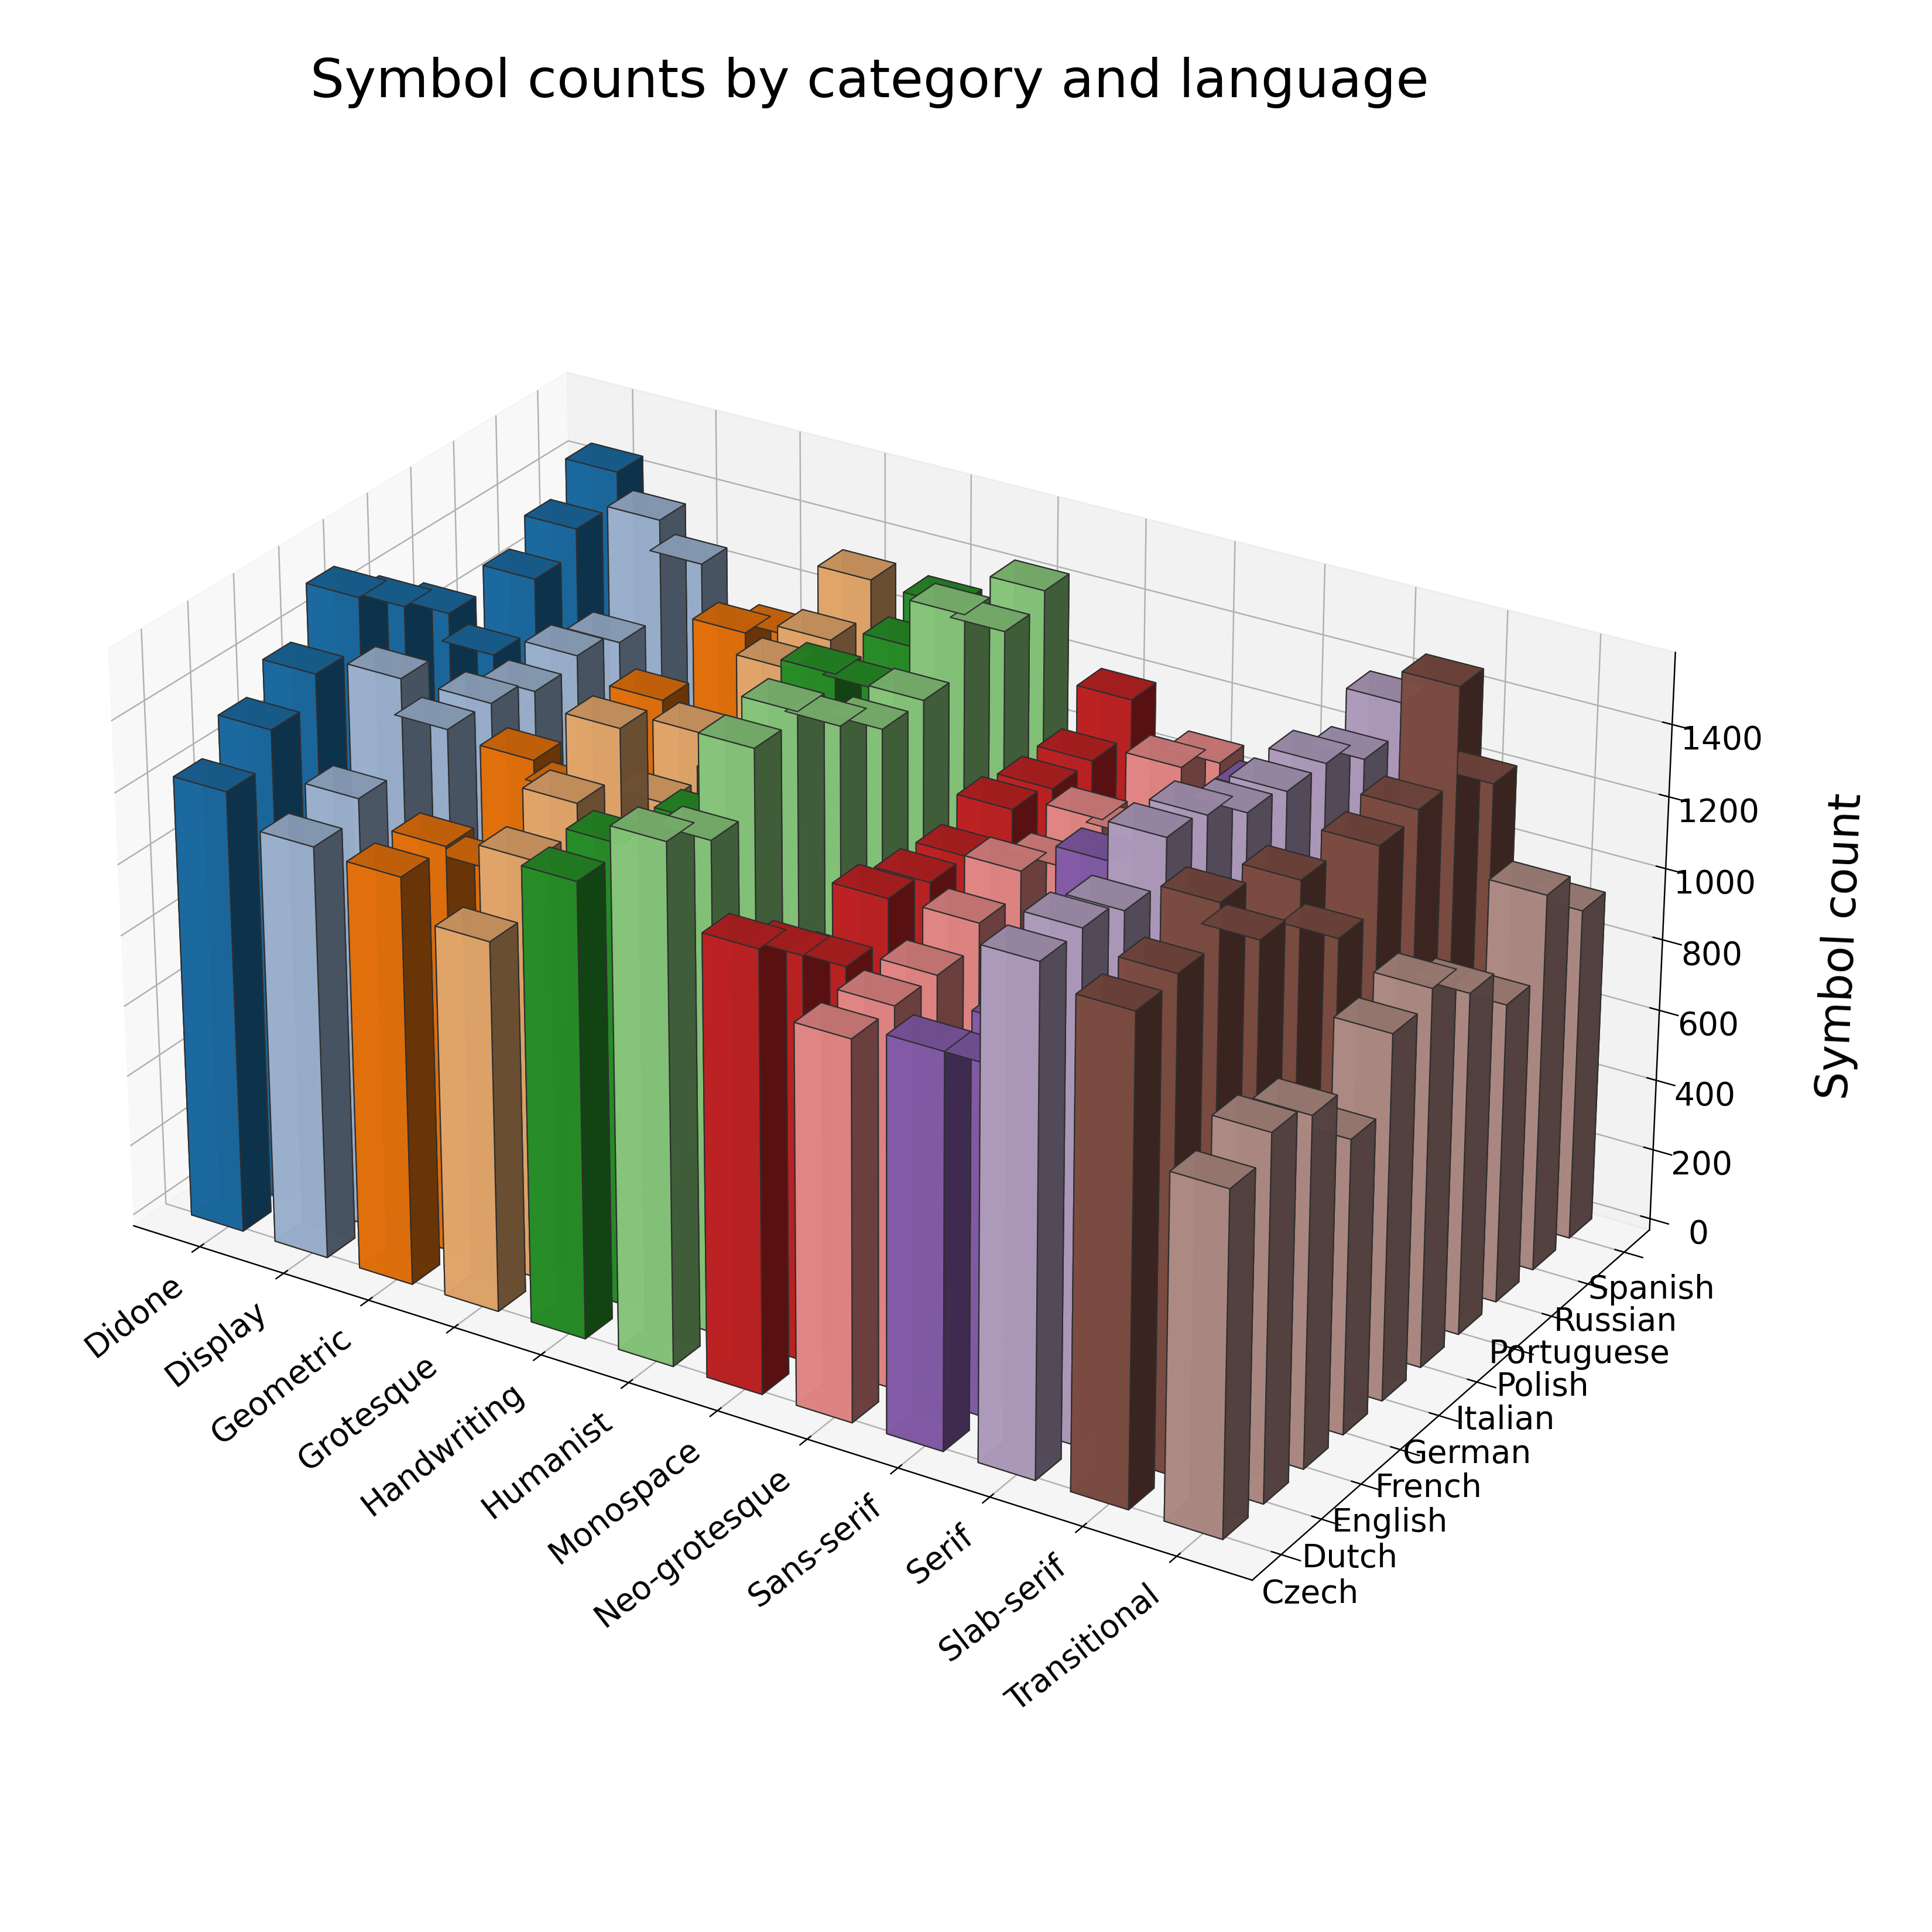
\includegraphics[width=\textwidth]{histograms/query-08-histogram-3d.png}
    \caption{Трёхмерная гистограмма по результатам запроса 8}
    \label{fig:query-08-histogram-3d}
\end{figure}

Итоговые значения показаны на двумерной и трёхмерной гистограммах.

\subsubsection{Запрос 9}

Для начертания $A$ и гарнитуры $B$ поменять формат с $C$ на $D$.

\[
\begin{aligned}
P_1 &= T.name=A \land FF.name=B,\\
P_2 &= F_o.name=C \land F_n.name=D,\\
X &= T \bowtie FF \bowtie F_o \times F_n,\\
Q &= \sigma_{P_1 \land P_2}(X),\\
R_9 =
\operatorname{update}_{T.id\_Format=F_n.id}(Q).
\end{aligned}
\]

Текст запроса~9 приведён в листинге~\ref{lst:query-09}, результат выполнения показан на рисунке~\ref{fig:query-09-result}, схема плана выполнения --- на рисунке~\ref{fig:query-09-plan}.

\captionof{listing}{Запрос 9}
\label{lst:query-09}
\vspace{-10pt}
\inputminted[linenos, numbersep=10pt, firstnumber=1, fontsize=\small]{sql}{../src/queries/query_09.sql}

Запрос находит начертание $A$ в гарнитуре $B$, проверяет его текущий формат $C$ и меняет его на формат $D$. Через \mintinline{sql}{RETURNING} выводятся старый и новый форматы.

\screenshot[fig:query-09-plan][0.95]{img/query-09-plan.png}{План выполнения запроса 9}

План выполнения запроса 9 находит старый и новый форматы, затем соединяет начертание с гарнитурой и проверяет условия по названиям. После нахождения нужной строки PostgreSQL выполняет обновление, а оператор \mintinline{sql}{COMMIT} фиксирует изменение.

\screenshot[fig:query-09-result][0.75]{img/query-09-result.png}{Результат выполнения запроса 9}
